\begin{frame} \frametitle{\vspace*{0.5cm}Results: Late-time evolution of the interface}
  \begin{figure}
    \centering%
    \only<1>{
    %   \begin{tikzpicture}
    %   \node[anchor=south west,inner sep=0] (image) at (0,0) {
    %     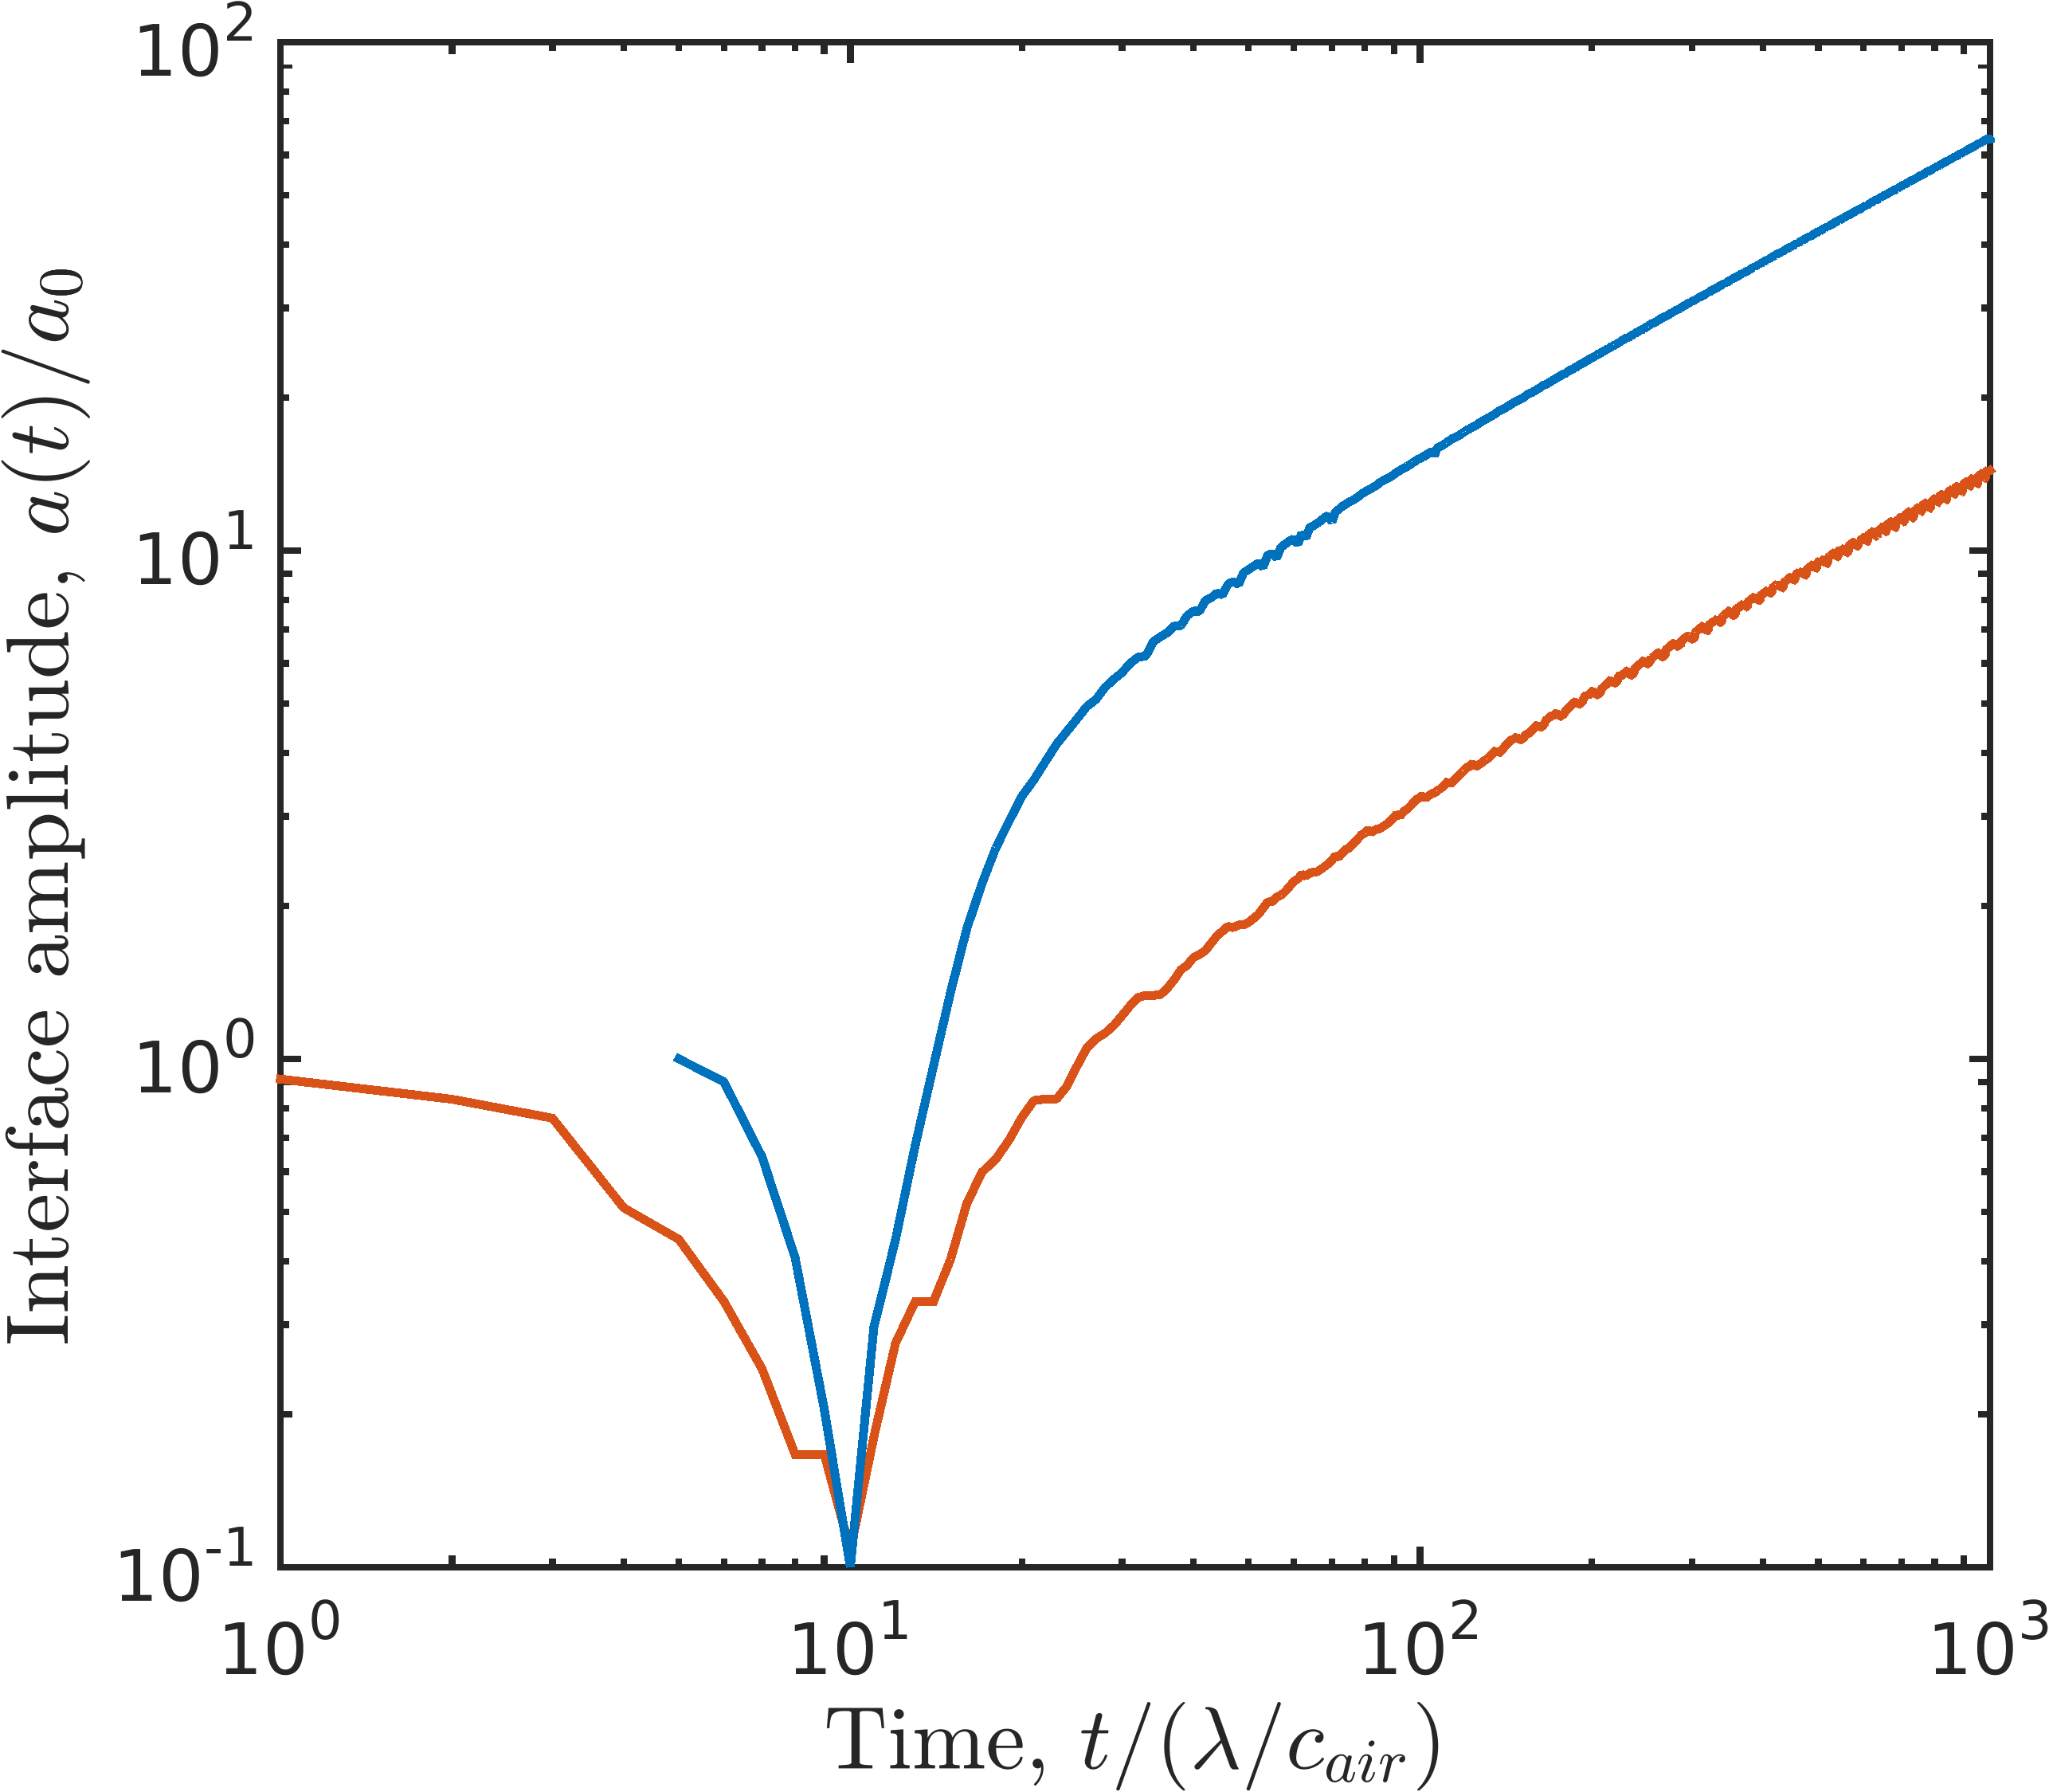
\includegraphics[width=0.6\textwidth]{../figs/lung_figs/interface_multi-amp_loglog_roe_t1000_nolines}
    %   };
    %   \begin{scope}[x={(image.south east)},y={(image.north west)}]
    %     \node[font=\footnotesize,right] at (0.4,0.7){ $10$ MPa};
    %     \node[font=\footnotesize,right] at (0.6,0.4){ $5$ MPa};
    %   \end{scope} 
    % \end{tikzpicture}
  }
    \begin{tikzpicture}%
      \node[anchor=south west,inner sep=0] (image) at (0,0) {%
        \only<1>{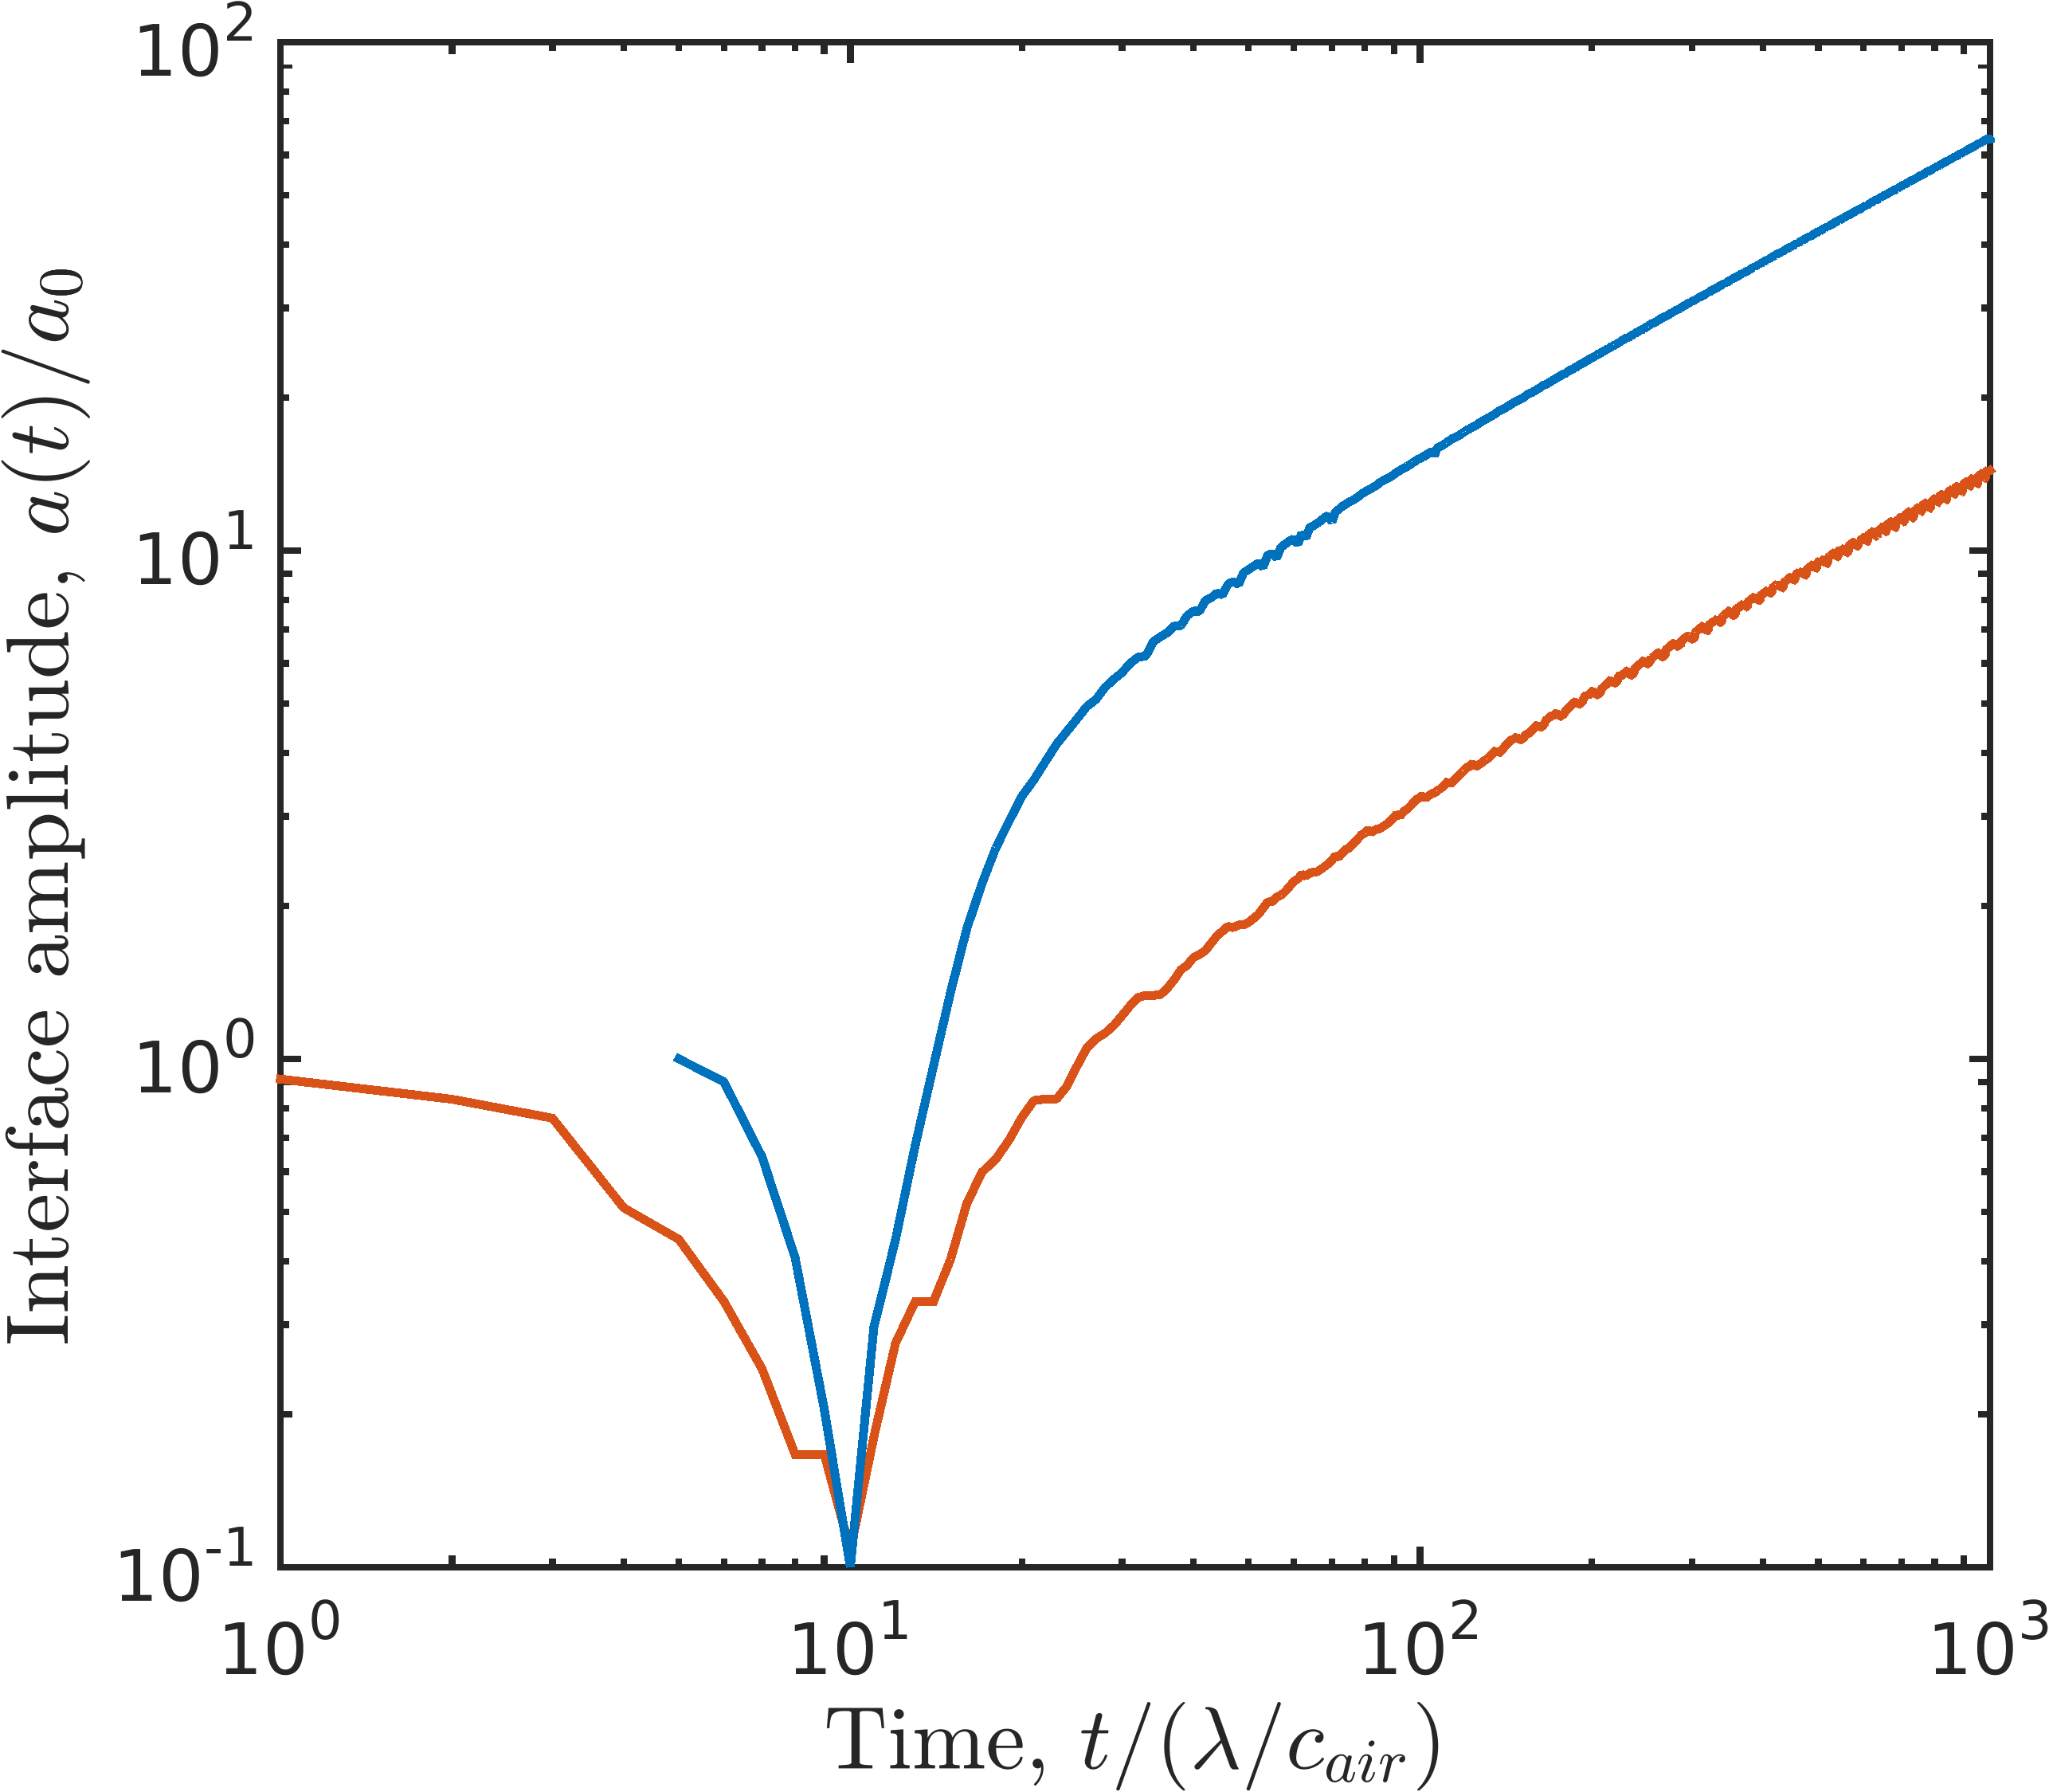
\includegraphics[height=0.54\textheight]{../figs/lung_figs/interface_multi-amp_loglog_roe_t1000_nolines}}%
        \only<2->{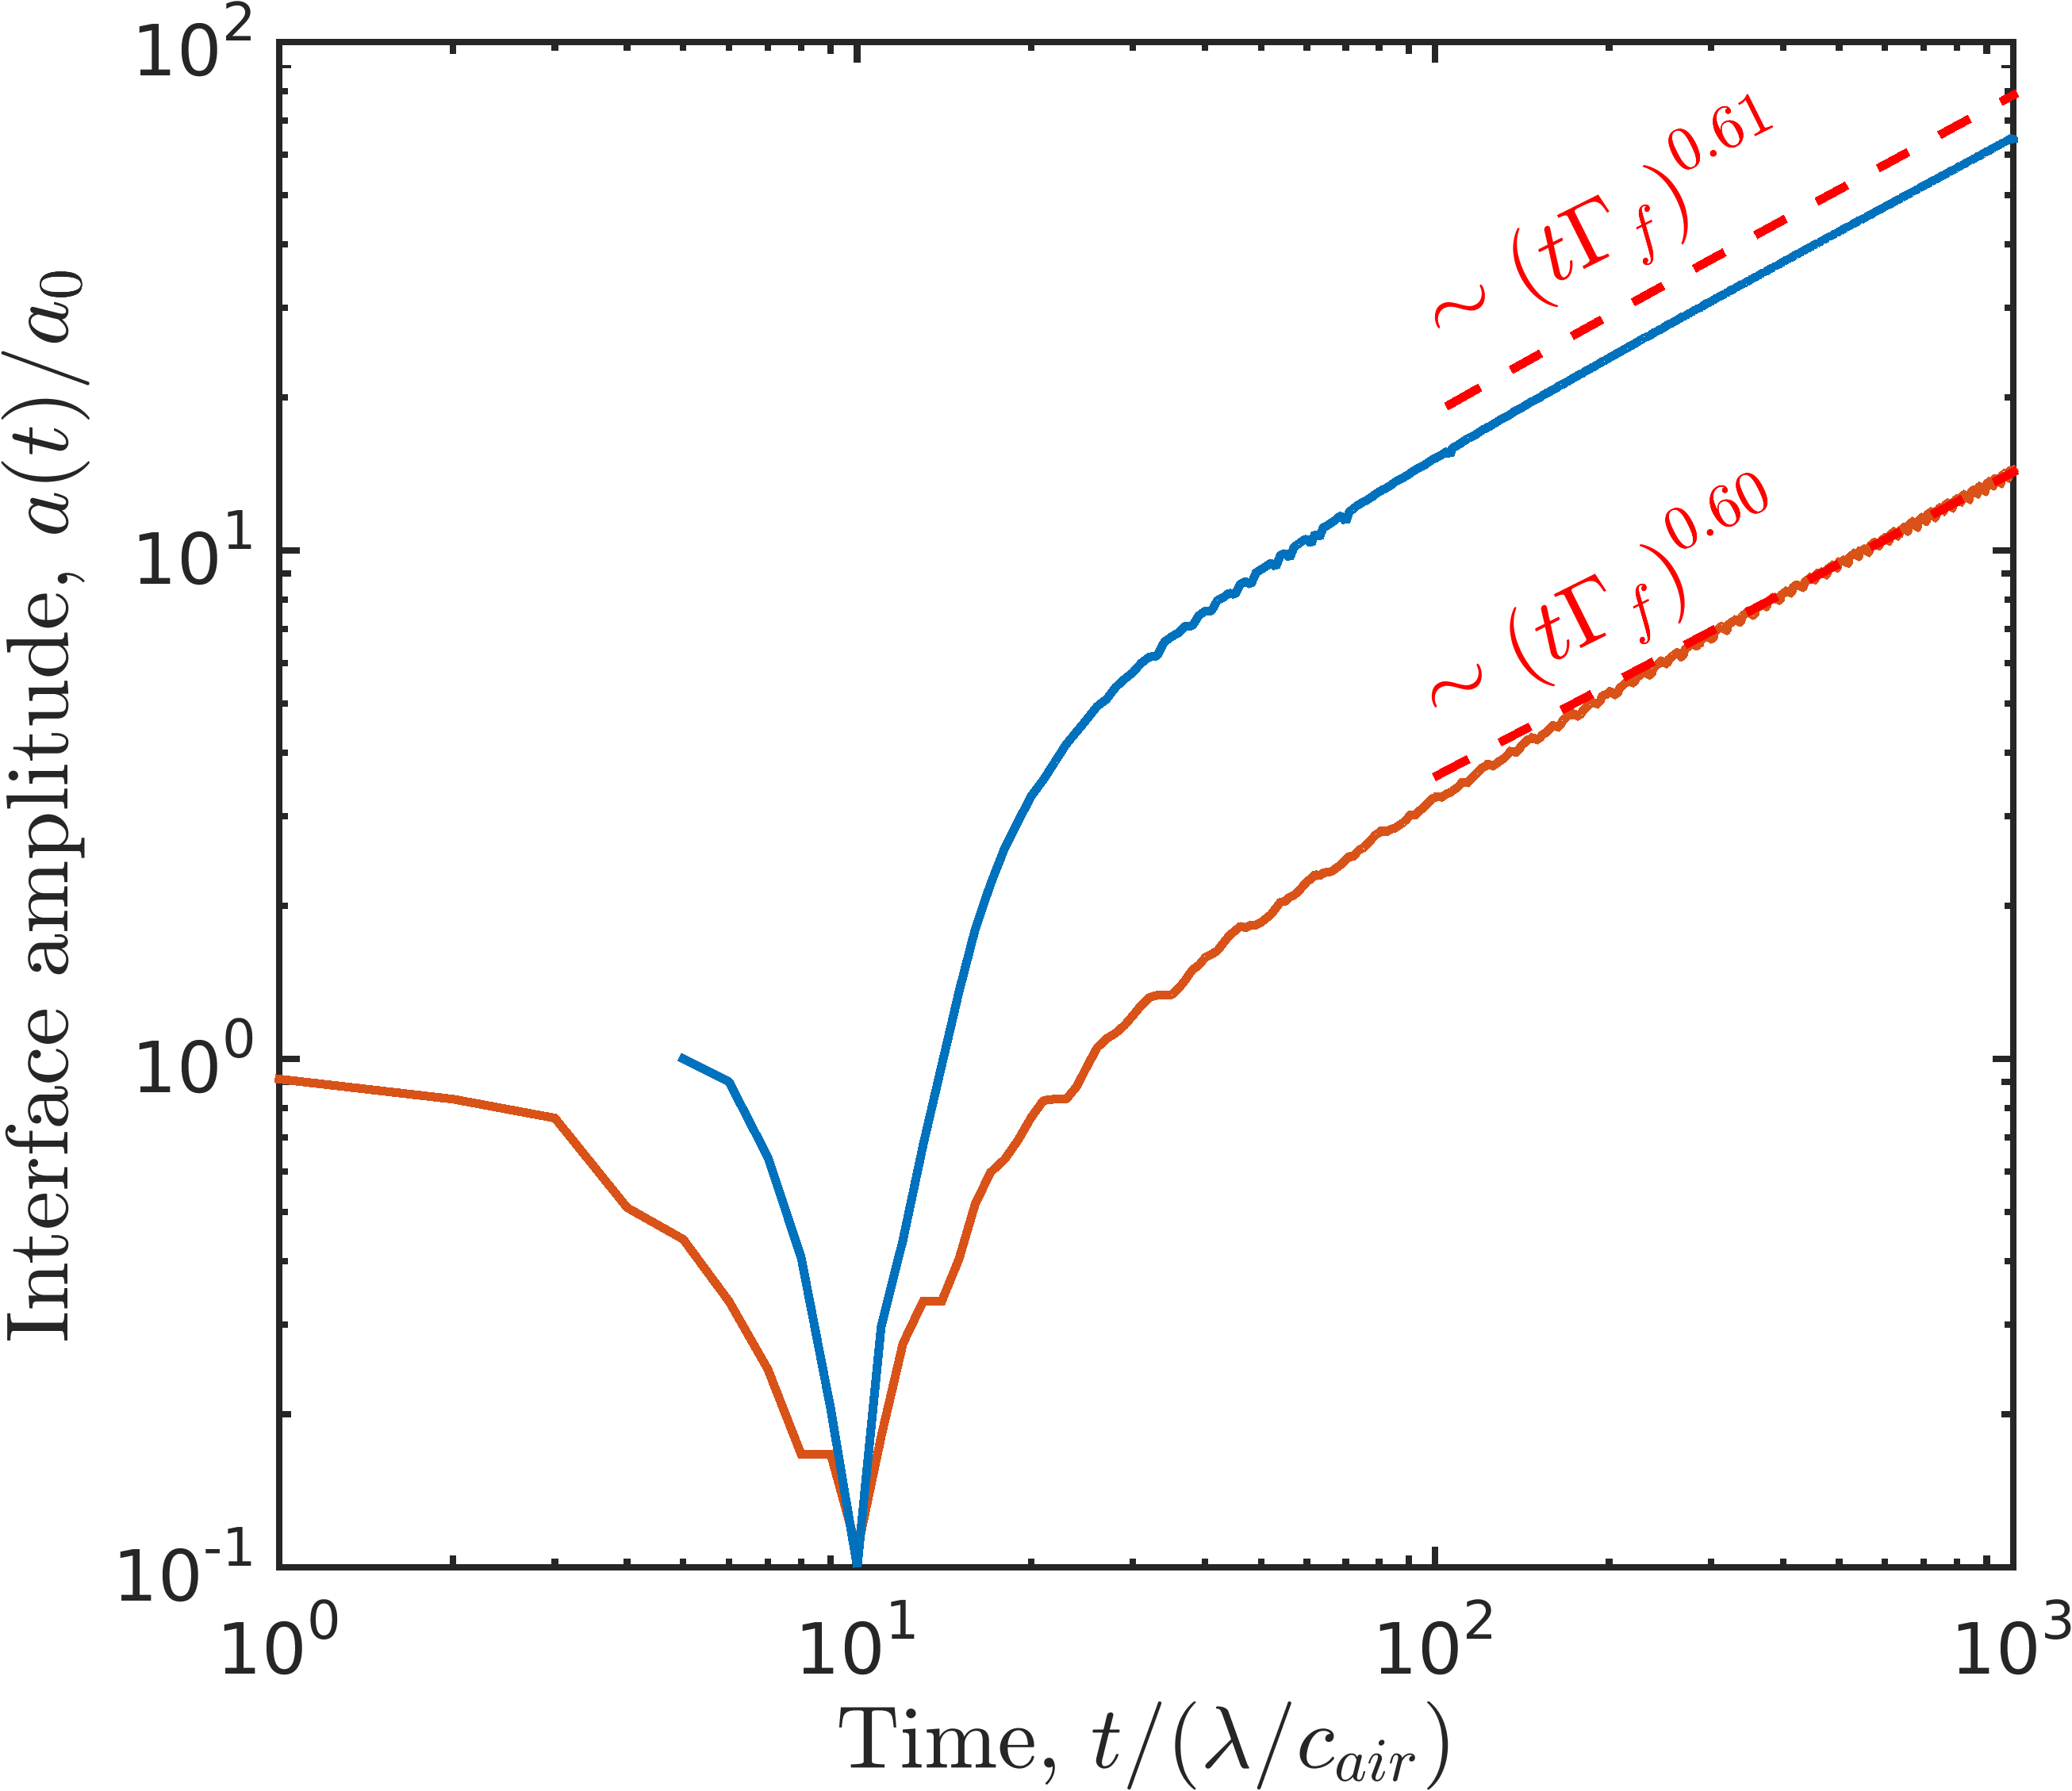
\includegraphics[height=0.54\textheight]{../figs/lung_figs/interface_multi-amp_loglog_roe_t1000}}%
      };%
      \begin{scope}[x={(image.south east)},y={(image.north west)}]%
        \node[font=\footnotesize,right] at (0.38,0.7){ $10$ MPa};%
        \node[font=\footnotesize,right] at (0.57,0.4){ $5$ MPa};%
      \end{scope}%  
    \end{tikzpicture}%
    \hfill%
    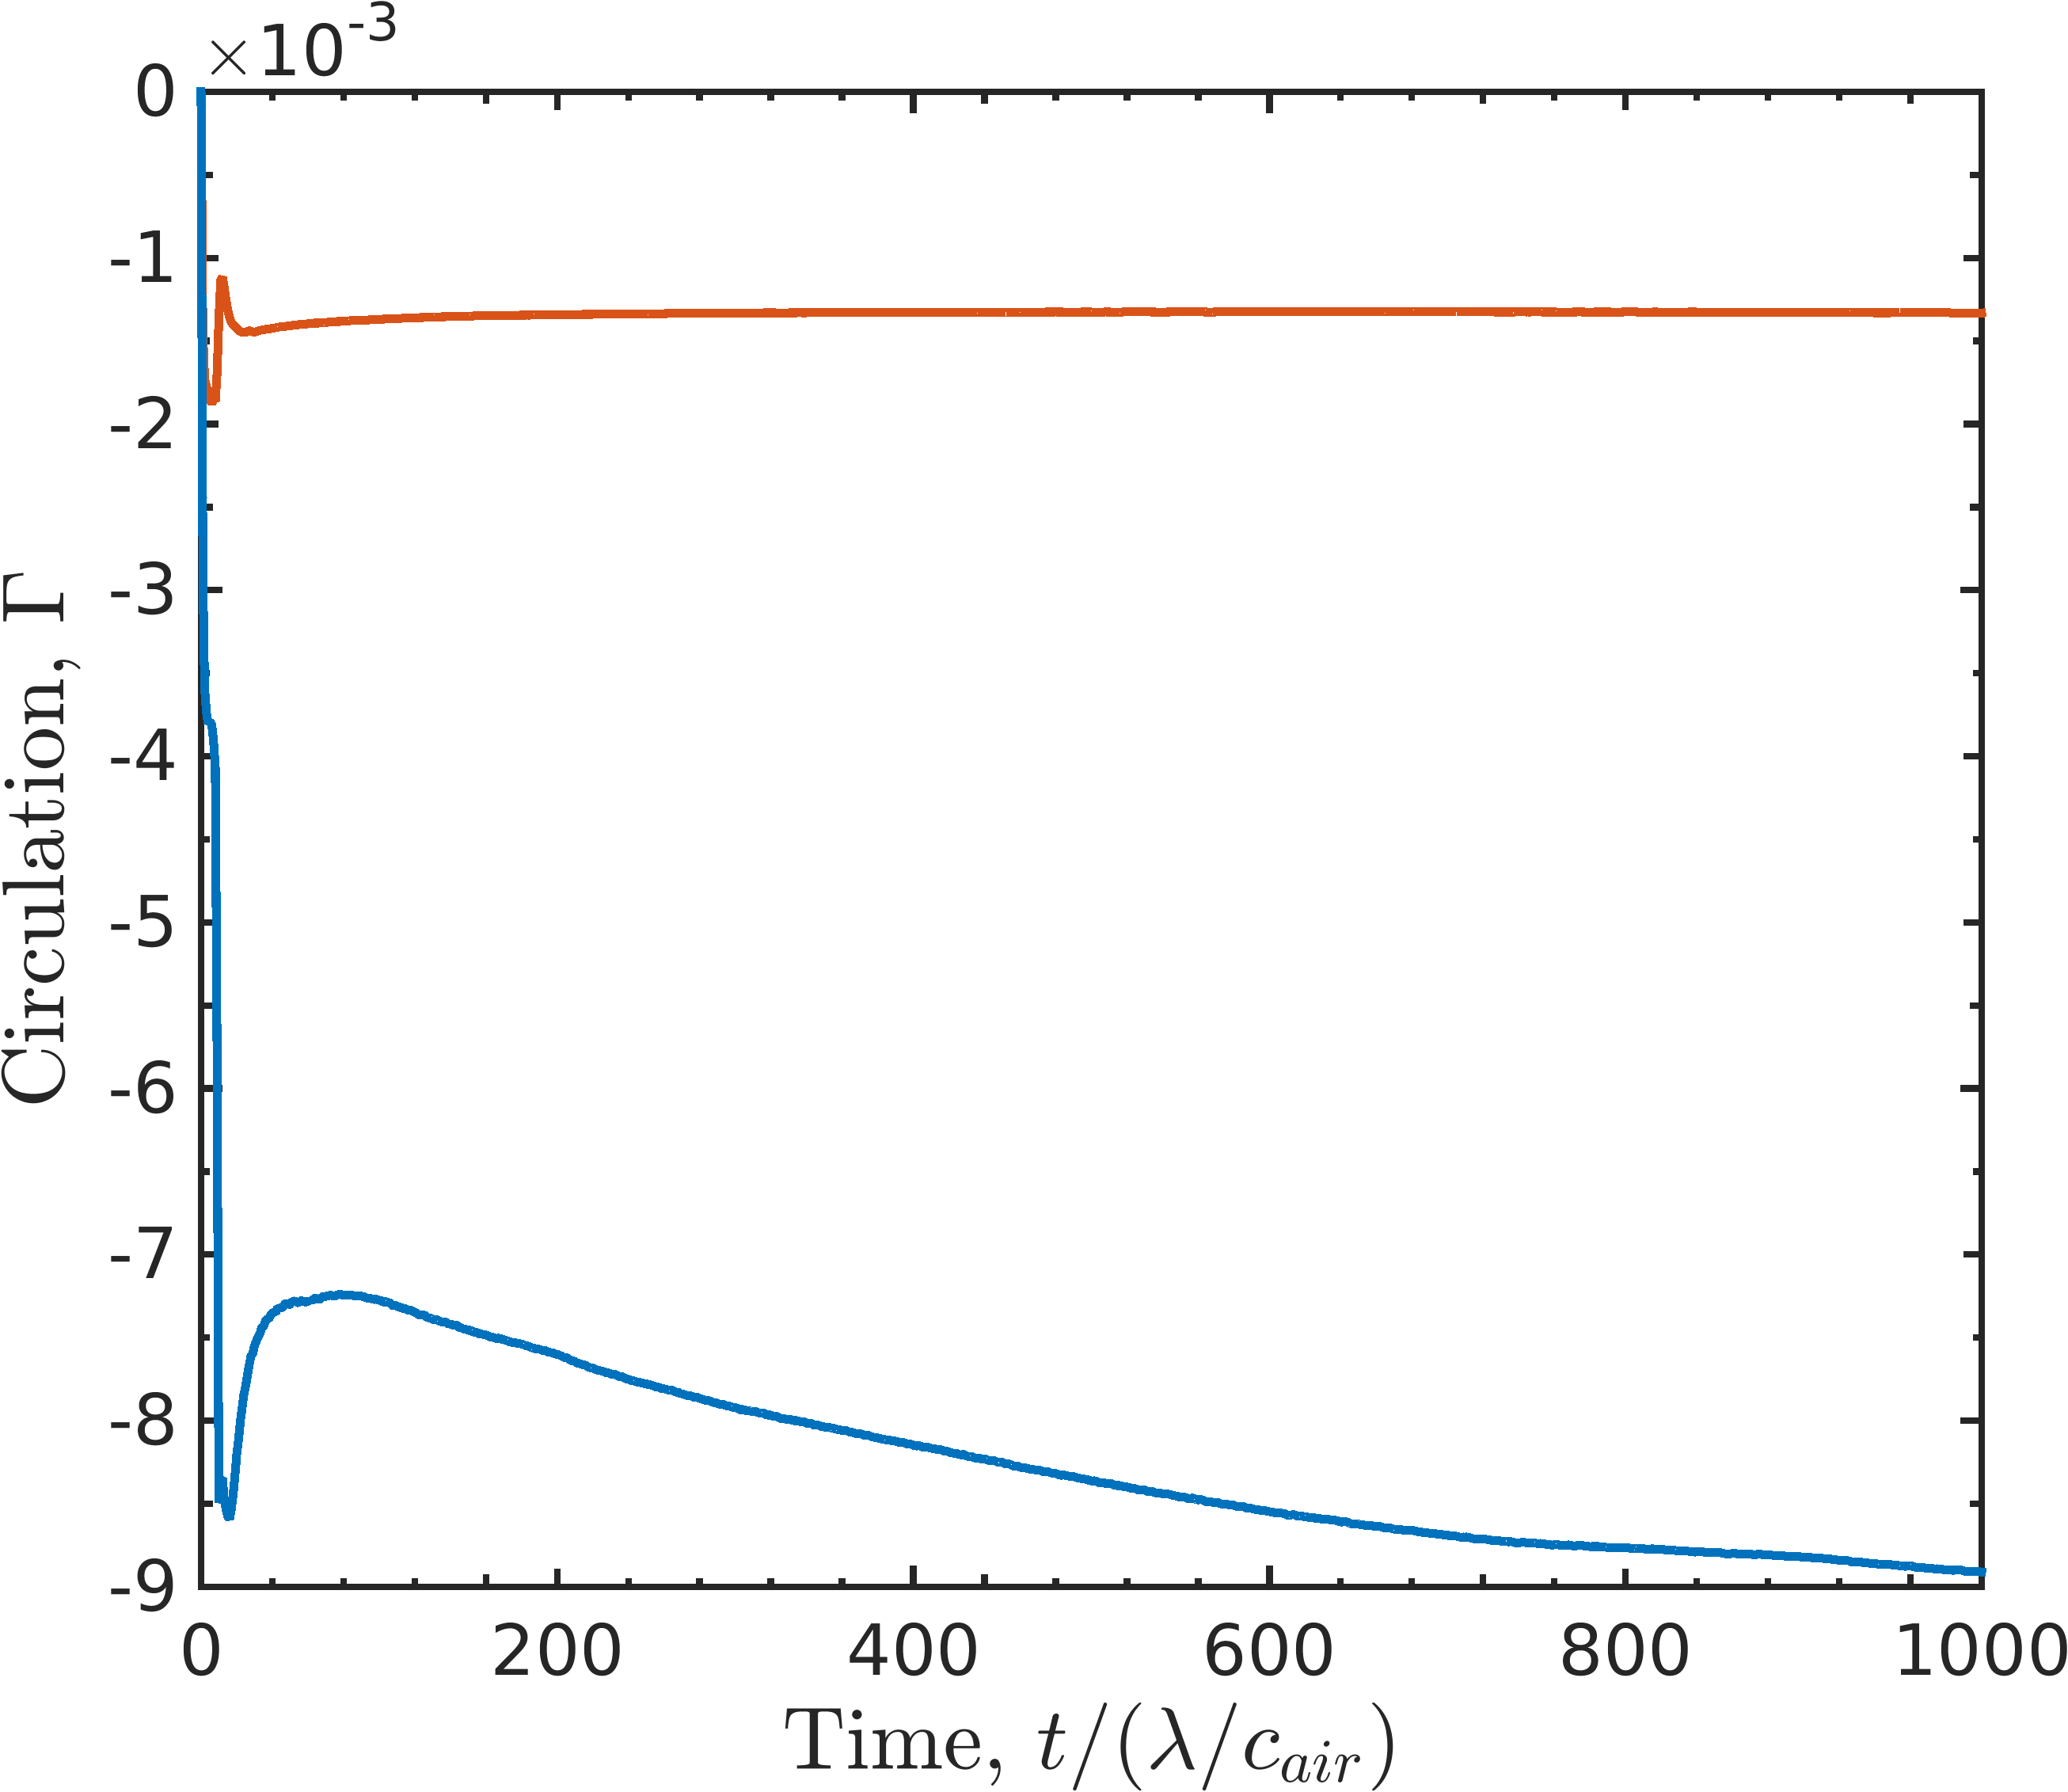
\includegraphics[height=0.54\textheight]{../figs/lung_figs/circulation_multi-amp_roe_t1000}%

    
  \end{figure}
  {\small
    From dimensional analysis, we expect a purely circulation growth of the interface perturbation to behave according to $a(t) \sim \sqrt{\Gamma t}.$
  }
\end{frame}
%%% Local Variables:
%%% mode: latex
%%% TeX-master: "../main"
%%% End:
